%introduce some nomenclature
\nomenclature[Y]{Percept}{A percept is an interpreted reading of the state of the environment, taken by the agent's sensor}
\nomenclature[Y]{Action}{An action is ...}
\nomenclature[Y]{State}{A state is ...}
\nomenclature[Y]{Utility function}{A utility function is a function that maps a sequence of states to a real number. It is used to give a value to the outcome of actions. }
\nomenclature[Y]{Performance Measure}{A performance measure is }
\nomenclature[Y]{MAS}{Multi-Agent System}

\subsection{Agency} \label{AgencySubsection}
An essential concept which is repeatedly referred to in this thesis is that of an \emph{agent}. The term "\textit{agent}" is an abstract one with no single definition universally accepted in the literature. Most definitions agree reasonably closely with the one provided in AI: A Modern Approach by Russell and Norvig: an agent is "\textit{anything that can be viewed as perceiving its environment through sensors and acting upon that environment through actuators.}"\cite{AIAMA}.  Figure\ref{fig:agent_env_interaction} helps to illustrate this concept. \begin{figure}
    \centering
    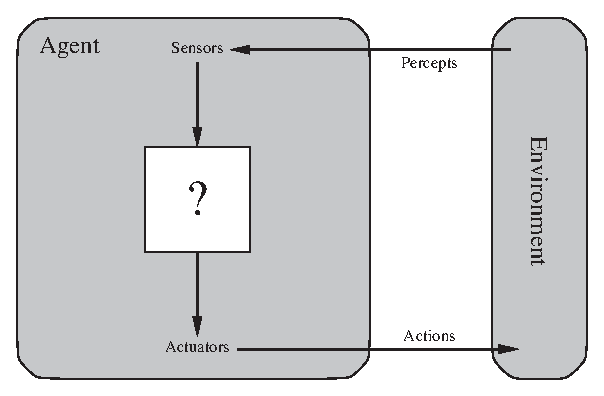
\includegraphics{Chapters/BackgroundKnowledgeAndRelatedWork/Figs/Vector/agent-environment.eps}
    \caption{Agent-Environment Interaction (Russell and Norvig)\cite[p.~35]{AIAMA}}
    \label{fig:agent_env_interaction}
\end{figure}
The box containing the question mark represents the agent's internal decision-making process, which generally speaking involves choosing an action, given the complete history of everything that the agent has perceived. The mapping from percept sequences to actions is described as the agent function. The agent function is an abstract notion; at a lower level an agent program implements the agent function, running on some physical system. A key concept in developing an agent program is rationality: "\textit{for each possible percept sequence, a rational agent should select an action that is expected to maximize its performance measure, given the evidence provided by the percept sequence and whatever built-in knowledge the agent has}"\cite[p.~37]{AIAMA}. This thesis is concerned with designing a system of agents that should exhibit rational behaviour.\newline
 

Russell and Norvig group agents into four common classes based on the design of the agent function\cite[p.~47]{AIAMA}: 
\begin{enumerate}
    \item \textbf{Simple reflex agents}: These agents select actions to take by ignoring the percept history to date, with the exception of the most recent percept.
    \item \textbf{Model-based reflex agents}: These agents have an internal state that depends on the percept history and is updated using new percepts. Updates occur using a model of the world.
    \item \textbf{Goal-based agents}: These agents are an extension to model-based reflex agents. They have some information about whether they have reached a "goal" state, which is desirable. The agent can choose actions to take based on the model. \note{Define what a goal state is.}
    \item \textbf{Utility-based agents}: A utility function is used as an internal performance measure in order to select actions. This allows an agent to pick among actions that may not immediately lead to a goal state.
\end{enumerate}
Recent work in the field of AI has strongly focused on learning agent architectures, which is a superset of all of the above agents. The key difference between the agent types listed above and a learning agent is that a learning agent has the ability to improve its performance through time independently. Its decision making process is not necessarily static and can change beyond its initial programming. An explanation of the architecture of a learning agent can be found in Russell and Norvig \cite[p.~55]{AIAMA}. Implementing each of these different types of agents requires varying degrees of effort. Depending on the problem, different architectures may be more or less suited, which suggests that fully understanding the problem that is attempted to be solved is of fundamental importance when designing an agent.

\subsection{Multi-Agent Systems}
Analogous to the definition of an agent, there is no universally agreed-upon definition of a \emph{Multi-Agent System} (MAS). A definition is provided in a field review paper by Stone and Veloso: "\textit{Multiagent Systems (MAS) is the subfield of AI that aims to provide both principles for construction of  complex  systems  involving  multiple  agents  and  mechanisms  for  coordination  of  independent  agents’ behaviors}" \cite{Stone2000MultiagentPerspective}. While the design of individual agents tends to focus on maximising a performance measure, the design of a multi-agent system is rather more multi-faceted. Weiss \cite{MAS:AModernApproachToDAI} notes that it is almost always oriented towards answering the question of "\textit{when and how to interact with whom}". Multi-agent systems have been proposed as a solution to many problems that modern AI attempts to tackle for some of the following reasons, which are outlined in more depth in \cite{Stone2000MultiagentPerspective}: 
\begin{itemize}
    \item Some problems by definition can be described as a multi-agent system. An example is an organization that may want to model it's internal affairs with a single system. The different departments have their own sub-systems that have differing priorities and capabilities; their interactions naturally can be thought of as interactions between independent agents, in accordance with the definition provided at the start of this section.
    \item The accomplishment of a task can be expedited significantly by using multiple agents. Multi-agents systems are part of the field of Distributed Artificial Intelligence (DAI) and so problem domains that decompose into several independent tasks that can be handled by separate agents can benefit from their use. The problem of efficient task allocation in multi-agent systems has been well-studied in the literature\cite{Gerkey2004ASystems}. 
    \item Robustness is an often-cited benefit of multi-agent systems. Distributed control means that failure of a single agent (mechanical or otherwise) may be tolerated.
    \item Multi-agent systems are often more scalable than single-agent systems. The necessary modularity of multi-agent systems means that adding new agents to the system can often be a solution to a more difficult problem, rather than adding new capabilities to a monolithic system. 
    \item The modularity of multi-agent systems means that the design and programming of them may be simplified. For example, rather than solving a multi-objective problem with a single agent, a single-objective problem may be solved with multiple agents. A result of this is that multiple cheap robots may be used to outperform a single, expensive robot \cite{Grabowski2000HeterogeneousExploration}.
\end{itemize}
\par

